\chapter{Implementation}
This chapter aims to present the reader with explanation of the key implementation aspects. These include major challenges, decisions and problems that have been encountered and taken during the course of this project. I have tried to avoid going into too much technical details except where this is essential and provides the reader with better insight and understanding of the material.

\section{iBus AVL Data}
The data that is used for this project is provided by the Technical Service Group (TSG) at TFL. The data consists of comma separated value files. There is an individual file for every different bus operator which contains the data for all buses currently operated by this company. Initially every bus in the network would transmit its unique identification number and GPS coordinates approximately every 30 seconds \cite{Hounsell201276}. This information is then preprocessed by a central server. This results in more information being derived as the central server has knowledge of the whole network and the bus schedules and headways. This results in the CSV feed files that have been provided to us for this project. An example of the content of the raw feed file and a formatted version is presented in section A.4 of Appendix A. Below I have provided a detailed explanation of each field in these files.
\begin{itemize}
	\item \textbf{Vehicle Id} - this is a unique id of the vehicle.
	\item \textbf{Bonnet Code} - this is the bonnet code of the bus.
	\item \textbf{Registration Number} - this is the number of the registration plate of the bus. 
	\item \textbf{Time of Data} -  this refers to the date and time of when this data is received from the respective vehicle.
	\item \textbf{Base Version} - this the version of the system that is run by the respective bus.
	\item \textbf{Block Number} - this is the block number on which the vehicle is running
	\footnote{\label{loggedProperly}This is only valid when bus is properly logged.}$^{,}$\footnote{\label{routeVariant}Not available in route variant.}.
	\item \textbf{Trip Id} - stores the internal trips id\footnotemark[\ref{loggedProperly}]$^{,}$\footnotemark[\ref{routeVariant}].
	\item \textbf{LBSL\footnote{London bus services limited \cite{lbsl}} Trip Number} - this is LBSL trip number\footnotemark[\ref{loggedProperly}].
	\item \textbf{Trip Type} - the type of the trip\footnote{1:From depot to start stop of the block; 2:To new starting point;  3:Normal trip with passengers; 4:From the last stop of the block to the depot; 5:Without passengers; 6:Route variant; 7:Vehicle not logged in either block or route}.
	\item \textbf{Contract Route} - the route name\footnotemark[\ref{loggedProperly}]$^{,}$\footnotemark[\ref{routeVariant}].
	\item \textbf{Last Stop ShortDesc} - this is the lbsl code of the last stop visited by the respective bus\footnotemark[\ref{loggedProperly}]$^{,}$\footnotemark[\ref{routeVariant}].
	\item \textbf{Schedule Deviation} - this is the standard deviation from the schedule, calculated using the bus position telegram, for the respective bus\footnotemark[\ref{loggedProperly}]$^{,}$\footnotemark[\ref{routeVariant}].
	\item \textbf{Longitude} - this is longitude of the place from where the vehicle is sending the telegram\footnote{\label{gps}GPS raw data divided by 3,600,000.}.
	\item \textbf{Latitude} - this is latitude of the place from where the vehicle is sending the telegram\footnotemark[\ref{gps}].
	\item \textbf{Event Id} - the last event Id.
	\item \textbf{Duration} - currently not being populated.
\end{itemize}

The information we are interested is the deviation from the schedule. This value is calculated the same way for both low\footnote{Less than 5 buses per hour.} and high\footnote{5 or more buses per hour.} frequency buses by knowing the bus schedule. It must be noted that it is possible vehicles would start the route already with some deviation from the schedule.

%Include a sample of the data and explanation of all fields
%Explain what the schedule deviation value means
%Include discussion on how the network is represented and the source of the file - TFL open data
%iBus system generate very short telegram messages with the bus location \cite{Hounsell201276}. This information is then processed on a server and more information is calculated and derived.
%The data that has been provided by Technical Service Group (TSG) at TFL for this project consists of preprocessed iBus feeds. This feeds currently are being generated every 5 minutes. Each file consists of the following fields:
%The information we are interested is the deviation from the schedule. This is calculated by knowing the expected arrival time of the bus at a stop from the schedule and is compared to the observed time. This value is calculated the same way for both low and high frequency buses(Low frequency buses are supposed to run according to a fixed schedule (e.g. a bus should arrive at stop at predefined time) and usually routes which have less than 5 buses an hour. High frequency bus routes should maintain headways - this meaning a bus should be arriving at stop at predefined intervals (e.g. each 2 minutes)). More about the supplied data for this project would be covered in the requirements section.
%Key property of time series data is stationarity. This means that the behaviour of the time series data does not change over time. In our case the data generally speaking the time series data is not stationary. However if we consider short window size it might be possible to treat the data as close to stationary.

\section{Prototypical Tool}
The system we have developed as a prototype which to satisfy our aims consists of two sub systems. These are the disruption engine which address the first aim of detecting disruptions in the bus network and a web front end application which to visualise the calculated disruptions. Below I have presented the major implementation decisions and challenges that were faced during the development of this system.

\subsection{Disruption Engine}
The disruption engine is implemented based on the design given in the previous chapter. The main implementation language used to the implementation is Scala. Scala is both functional and object oriented language. It is a type-safe Java Virtual Machine (JVM) language. This means that it is compatible with existing Java code which allows for reuse of existing Java libraries. Scala was first introduced back in 2003, however it has been only in the past few years that it had gained more popularity. In addition Scala enables the programmer to write more concise and clear code than Java. The decision of using Scala has also been influenced by the fact that I have good knowledge of the object oriented programming paradigm as well as experience in Java. This allowed me to quickly learn Scala and put it into use.

The disruption engine need to have an accurate internal representation of the bus network. TFL's bus network and any other bus network usually consists of bus routes. Each bus route often has multiple runs (directions - e.g. inbound and outbound). In turn each run consists of a sequence of bus stops that the bus passes through. In addition to these typical bus network components for our implementation we also have the notion of section. By this we mean a pair of consecutive bus stops along a given run of a given route [FIGURE EXAMPLE].

Our tool makes use of a PostgreSQL database for storing all configuration parameters and also for storing the required information for the bus network representation. In figure A.8 in Appendix A I have presented the database model on which the database is based. This database is also means of providing the user interface web application with the output of the engine (the disruption that have been detected and their details). I have decided to use PostgreSQL as it is advanced open source relation database management system. PostgreSQL has very good document and community support which big advantage for any technology. One other advantage for using PostgreSQL for our implementation is that it ensures reliability and data integrity. Also it supports Listen and Notify functionality which could be used for real-time updating of the web application along with Server Sent Events (SSE).
	
%Why have I have decided to use database vs flat file data store. Pros and cons
%Why postgresql. Reference to the database model
%Explanation and discussion of the database model.

%However as other research has pointed out \cite{1251929} calculating travel time as measure for congestion is difficult task and it is very dependable on the environment and its conditions (e.g. weather, time of day, public demand etc.). For this reason and because of the data available this project would not try to measure disruptions by calculating travel time or bus speeds.TFL has provided us with example of the AVL data which among other things contains a the GPS coordinates of the bus at a given point in time and preprocessed deviation from the schedule value. For the rest of this chapter we assume this value is accurately calculated and that we would receive this value for each bus in the network at some regular interval. The provided data is discussed in further details in Chapter 5.
%For this project we monitor and measure the schedule deviation value as calculating the congestion is very challenging and still not very well understood in the case of arterial urban traffic.
%However from the literature \cite{1251929} we can see that it could be difficult to precisely define what we mean by congestion in a transport network. It seems that congestion could mean various things to different studies and people.
%What is the general approach I have taken
%WHAT ARE THE CHALLENGES AND HOW WERE THEY OVERCOMED
\subsubsection{Bus Network representation}
In order for the engine to have full bus network representation it requires information of the bus routes and the bus stops in the network. This information is freely available to anyone on TFL website [REFERENCE]. It consists of two csv files, one containing information on all bus routes and one for all bus stops in the network. The bus file contains a list of bus routes respectively has a one or more runs which consists of sequence of bus stops.
In our implementation we assume that this information is preloaded in to the database. This pre load consists of simply extracting the information from the csv files obtained from TFL website into the respective tables (BusStops and BusRouteSequences). In addition to this we need to pre load also the sections which will allows us to store individual section information. Then once the engine is started it would read and load from the database all bus routes and respective sections. This results in the BusNetwork class storing a HashMap which maps a bus route name to the corresponding Route object. In turn the Route class keeps a list of all runs that it has. BusStop information (apart from the bus stop lbsl code which we use as an id) is only loaded from the database on request. This whole initialisation process happens only once throughout the execution of the tool and it is the first thing to happen along with reading the Environment parameters.

\subsubsection{Monitoring and processing new feeds}
Once the system is initialised the tool would continuously monitor (a specific directory) for new feeds being written. Once new feed files are detected they are picked up and processed by the engine. The processing consists of extracting the data of interest and calculating the time lost by buses on average for each section. Extracting the data means reading the csv feed file line by line. Each line would be a data (observation) for a given bus thus we associate each observation with the route that is currently logged on. Once the observations are extracted they are sorted by the time of the data field and any data that is older than a given predefined threshold (e.g. 2 hours - this is configurable) is discarded. Once a feed file is finished processing it is moved to a predefine processed feed directory. This completes the feed file processing step.
	
\subsubsection{Bus network state update}
Once feed processing has finished the system need to update the bus network state. This consists of few steps. First we need to calculate the lost time per section. This process is done iteratively for every route in the network that has active buses (readings have been transmitted in some predefined interval of time). Each bus observation is then taken on a given route (see Figure 1). At least two or more observations are required in order to calculate the time loss for a section. In the example below we can take the first reading x\textsubscript{1} and the second reading x\textsubscript{2}.
The difference in the schedule deviation between x\textsubscript{2} and x\textsubscript{1} is then calculated. Lets assume this difference is 3 and we can see that reading x\textsubscript{1} has been send from the first section of the route and reading x\textsubscript{2} from the the third section of the route. This means that the bus has lost 3 minutes between these two points on the route. However we cannot know for sure which section or sections have caused this loss and we can only distribute this loss equally between the three section. This means that each of section 1, 2 and 3 would be assigned 1 minute of loss. If we take however the case of reading x\textsubscript{3} and x\textsubscript{4} we can be very confident that the loss has occurred in section 5. Doing the above steps for each bus on a route we end up with a list of values representing the time loss and the time when this has occurred. The next step is to calculate the weighted moving average of this data. We do this by taking the list for each section and sorting it by the time of the observation (e.g in the above example section 1, 2 and 3 would have time of the data equal to the x\textsubscript{2} observation). Then we calculate the weighed moving average by assigning the oldest data weight of 1 and the newest data weight of n (n is the number of data entries of a section). Calculating the weighted moving average instead of a simple average we put more weight and the newer data and also help dampen the effect of a single irregularity (e.g. a bus has experienced a technical fault). If there is any section where buses are actually gaining time instead of losing thus resulting in a negative value we simply put 0 as we are only interested if there are any problematic sections.
\begin{figure}[ht!]
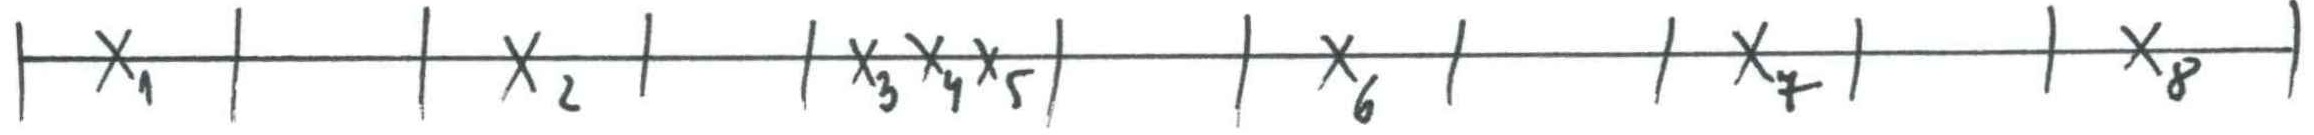
\includegraphics[scale=0.2]{Figures/figure1.jpg}
\caption{example 1 \label{overflow}}
\end{figure}
Once we have calculated the weight moving average time loss per section, we need to check if there are any sections that are of interested and need to be displayed (e.g. are there any disruptions). Here one problem arises as we need to take into account diversions. More details on this problem can be found in the section below. If we just ignore disruption we need to find if there is a number of consecutive sections which have their sum of the loss of time greater or equal to some predefined threshold (e.g. 20 minutes). For example in the example (see Figure 2) below we can see that section 5, 6 and 7 add up to 24 minutes of delay and thus we output that there is a disruption between stops E and H. 
\begin{figure}[ht!]
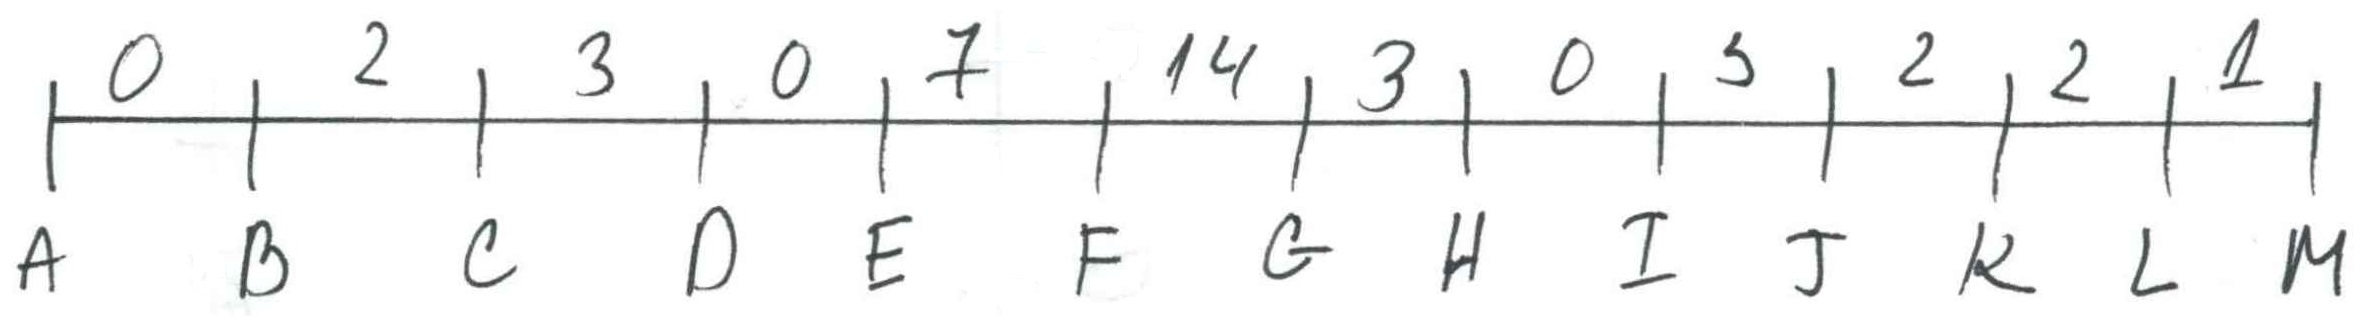
\includegraphics[scale=0.2]{Figures/figure2.jpg}
\caption{example 2 \label{overflow}}
\end{figure}
We have to limit the number of consecutive section we look at a single time as for example we consider the below case (see Figure 3). 
\begin{figure}[ht!]
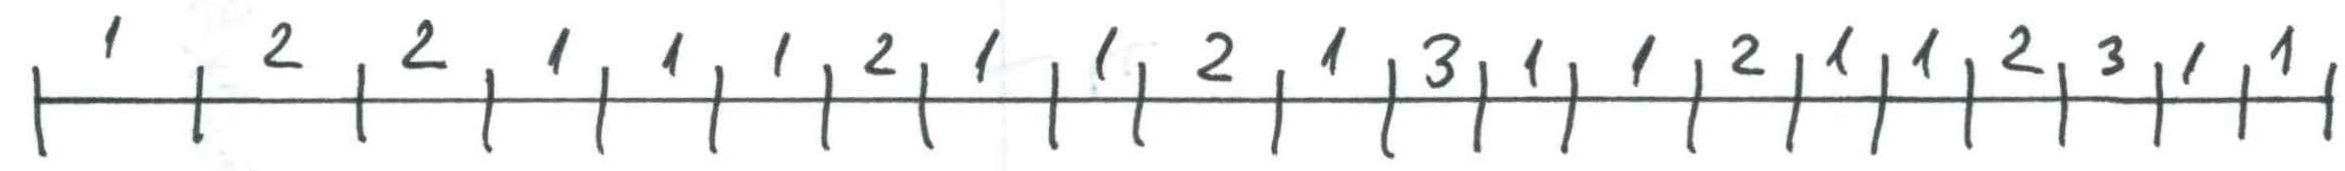
\includegraphics[scale=0.2]{Figures/figure3.jpg}
\caption{example 3 \label{overflow}}
\end{figure}
We can have a long route run with very small loss of time per section (as in the below example of the order of 1/2 minutes) but overall they might add up to 20 or more minutes. This however does not represent a single problematic hotspot and is responsibility of the bus operators to manage such cases and not CentreComm. This is also the scenario where diversions become problematic. Every detected disruption  or one that has changes its state is updated and written to the database. This allows for the user interface to update itself with the latest information.

\subsection{Graphical User Interface}
The engine implementation described above address only half of our requirements. In order to fully meet the project goals we need to be able to visualise the detected disruption in the network. For this reason I have decided to implement the visualisation part of the system as a separate web application. The advantages of this approach are that this provides universal access to the information. We only need to deploy this application once and it can be accessed from multiple clients running different operating systems and even devices. I have decided to use Ruby running on Rails framework. The reason for this is its recent popularity and wide support in terms of third party libraries and community information and guides.

The Rails framework [REFERENCE] is full stack open source web framework implemented in Ruby. It is relatively easy to use and maintain and it support a wide range of software engineering paradigms and patterns. The main ones being Model View Controller (MVC), Don't Repeat Yourself (DRY), Convention Over Configuration (CoC) and the Active Record pattern \cite{fowler2003patterns}. I have also made use of Foundation Cascading Style Sheets (CSS) front-end framework. This framework has enabled quick prototyping as it has a rich library of predefined components. However its main advantage over some other similar frameworks is its notion of grid which allows for quick and easy implementation of responsive websites. Making the web application with responsive design allows us to reach more platforms and client systems with a single application. This allows us with little additional implementation effort and time to achieve results which look good on both large screens (desktop computers, laptops etc.) as well as small mobile devices (e.g. smart phones, tablets etc.). This framework also has the advantages of good support in terms of documentation and add-ons and it is lightweight. Sample of what the system user interface looks like can be seen in appendix A [REFERENCE TO APPENDIX].

The ruby on rails web application is implemented following the MVC pattern. In our case it consists of few simple models representing the corresponding database tables, controllers and a number of views (some of which are partials). The models are implemented as Active Records which provide interfaces to the respective database tables. They provide create, read, update and delete (CRUD) functionalities. The controllers are responsible for processing the client request by parsing and checking for any parameters, credentials where necessary and responding with the requested information. The responses are in most cases rendered views containing the requested information.

One important aspect of the user interface is how to update the disruption list in real time whenever there are changes. This is achieved by implementing Ajax short polling. This means that we use asynchronous JavaScript on the client side to make request to the server at predefined intervals. Alternative methods for implementing the updating of the list include Web Sockets, Ajax Long Polling, Server Sent Events (SSE). The main advantages of using Ajax short polling over Web Sockets and SSE are that Ajax Short Polling is supported by all major web browsers unlike SSE which lack Internet Explorer support and it is easy and quick to implement it. The drawback of using Ajax polling is that in order to achieve near real time update the clients will need to make frequent request to the server which wastes network and server resources. SSE is probably the best approach in this scenario as it establishes a persistent long-term connection on which the server is able to push new data once it becomes available to all connected clients. However SSE are not supported by Internet Explorer which is one of the main web browsers CentreComm staff use and also SSE require a concurrency enabled server. Web Sockets provide a persistent two way connection between the client and the server however in our case we are mainly interested in pushing new data from the server to the client. There is very little information the clients need to send to the server and thus we have excluded this approach as viable one.

The disruptions at any point in time are visualised in tabular form. This provides instant awareness of what the network state is to the CentreComm operators. Disruptions are prioritised by their severity and are color coded. Further details for disruption are displayed on request of the user. This includes a graph representation of the delay observed on each section along the disrupted route. On this graph the cumulative delay for this route is also visible. When hovered the graph displays details for this section including the start and end stop of it and the number of observations.

\subsection{Problems}
One problem that was encountered is that there is no explicit information in the data that has been provided if a bus is on diversion. Diversions vary greatly in terms of length of the diversion (few or many stops) and duration of the implemented diversion (e.g. it can last half an hour or few weeks/months). What happens is such cases is that the bus would still transmit its position however the centre iBus server would not be able to calculate the schedule deviation. When such readings are observed by the engine they would simply be ignored. This is problematic and our system only ignores it in the current prototype as failure in computing the schedule deviation could also be caused by the bus not being properly logged into the iBus system (e.g. bus taking a break at end of route). This means that we lose some accuracy especially for longer diversions as any lost time would be distributed along the sections which have not been observed (where the bus has been on diversion). This however could also be the case if a bus skips or fails to send data. Again this could be because of number of reasons (e.g. weak signal due to high buildings etc.).
Another problem with the available data is that we do lose some reading when the bus turns at the end of a run. We cannot simply assume that every bus would travel along a route from start to end and turn as there are occasions when buses are curtailed along the route. This can happen for a number of reasons including service regulation, heavy congestion/disruption along some sections of a route, bus driver going above the work hours allowed by law and more.
Another problem of the approach taken is that because the system relies on monitoring the schedule deviation value and it does not treat differently calculations where during the first observation the bus is ahead or schedule and when it is already behind. This means that it is possible that the bus driver is losing time on purpose for service regulations. Thus we can assume that our tool provides an upper bound of the disruption.
%The important factors to consider are the weights and the period/window size to use. We could also apply exponential smoothing on top of the WMA.
%Problems:
%The bus could have started the journey ahead of schedule and thus to intentionally be losing time.
%The buses could curtail anywhere on a route without notification
%The buses could be diverted (this could be short term or long term) it can also be for few stops or it could be a longer diversion.

%PROBLEM - some buses might skip transmitting data even if they are properly logged on
%Data available, data frequency, no knowledge when buses do curtail, not taking into account bus dwell time, bus drivers who are running ahead of schedule could be driving slower on purpose and thus. Tool gives an upper bound of the of the WMA lost time per section. 
